% Created 2018-02-23 vie 16:58
\documentclass[letterpaper]{scrartcl}
\usepackage[utf8]{inputenc}
\usepackage[T1]{fontenc}
\usepackage{fixltx2e}
\usepackage{graphicx}
\usepackage{longtable}
\usepackage{float}
\usepackage{wrapfig}
\usepackage{rotating}
\usepackage[normalem]{ulem}
\usepackage{amsmath}
\usepackage{textcomp}
\usepackage{marvosym}
\usepackage{wasysym}
\usepackage{amssymb}
\usepackage{hyperref}
\tolerance=1000
\usepackage{khpreamble}
\usepackage{epic}
\usepackage{eepic}
\usepackage{epsfig}
\usepackage{psfrag}
\usepackage{rawfonts}
\author{Kjartan Halvorsen}
\date{2018-02-20}
\title{PID exercises}
\hypersetup{
  pdfkeywords={},
  pdfsubject={},
  pdfcreator={Emacs 24.5.1 (Org mode 8.2.10)}}
\begin{document}

\maketitle

\section{A PID controller with anti-windup}
\label{sec-1}
The figure below taken from Åström \& Wittenmark shows a block-diagram of a PID controller with anti-windup.
\begin{center}
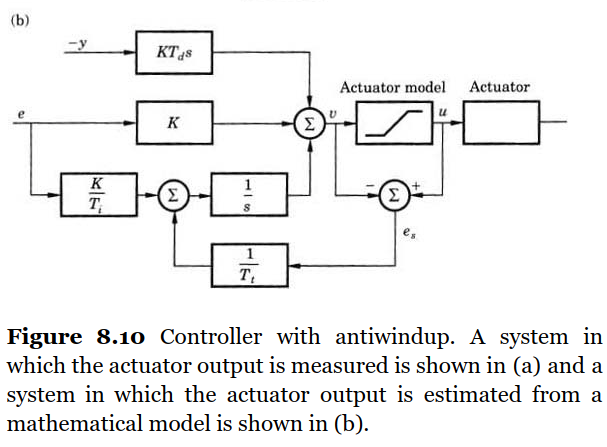
\includegraphics[width=0.51\linewidth]{../figures/fig8-10.png}
\end{center}
Consider the PID controller as having the output signal \(v(t)\) and three input signals: The control error \(e(t) = y_{ref}(t) - y(t)\), the output feedback signal \(y(t)\) and the output signal of the actuator model \(u(t)\). 
\begin{enumerate}
\item Determine the transfer functions in 
\[V(s) = F_y(s) Y(s) + F_e(s)E(s) + F_u(s) U(s). \]
\item Determine the pole(s) of the controller.
\item Determine the steady-state output of the controller for step input signals (all at once) \(Y(s) = \frac{\alpha}{s}\), \(E(s) = \frac{\beta}{s}\) and \(U(s) = \frac{\gamma}{s}\).
\item How should we interpret the steady-state value if the actuator is not saturating, so that \(u(t) = v(t)\)?
\end{enumerate}

\section{The effect of PID controller parameters}
\label{sec-2}
Assume a certain system being controlled by a PID regulator, \( U(s)=(K_P+K_I \frac{1}{s}+K_D s) E(s)\). In the figure below shows four step responses for the parameter
triples 
\begin{eqnarray*}
\begin{array}{cccc}
i) & K_P=1 & K_I=0 & K_D=0 \\
ii) & K_P=1 & K_I=1 & K_D=0 \\
iii) & K_P=1 & K_I=0 & K_D=1 \\
iv) & K_P=1 & K_I=1 & K_D=1 
\end{array}
\end{eqnarray*}
Match each one of the parameter triples to one of the step 
responses. Justify your answer!

\begin{center}
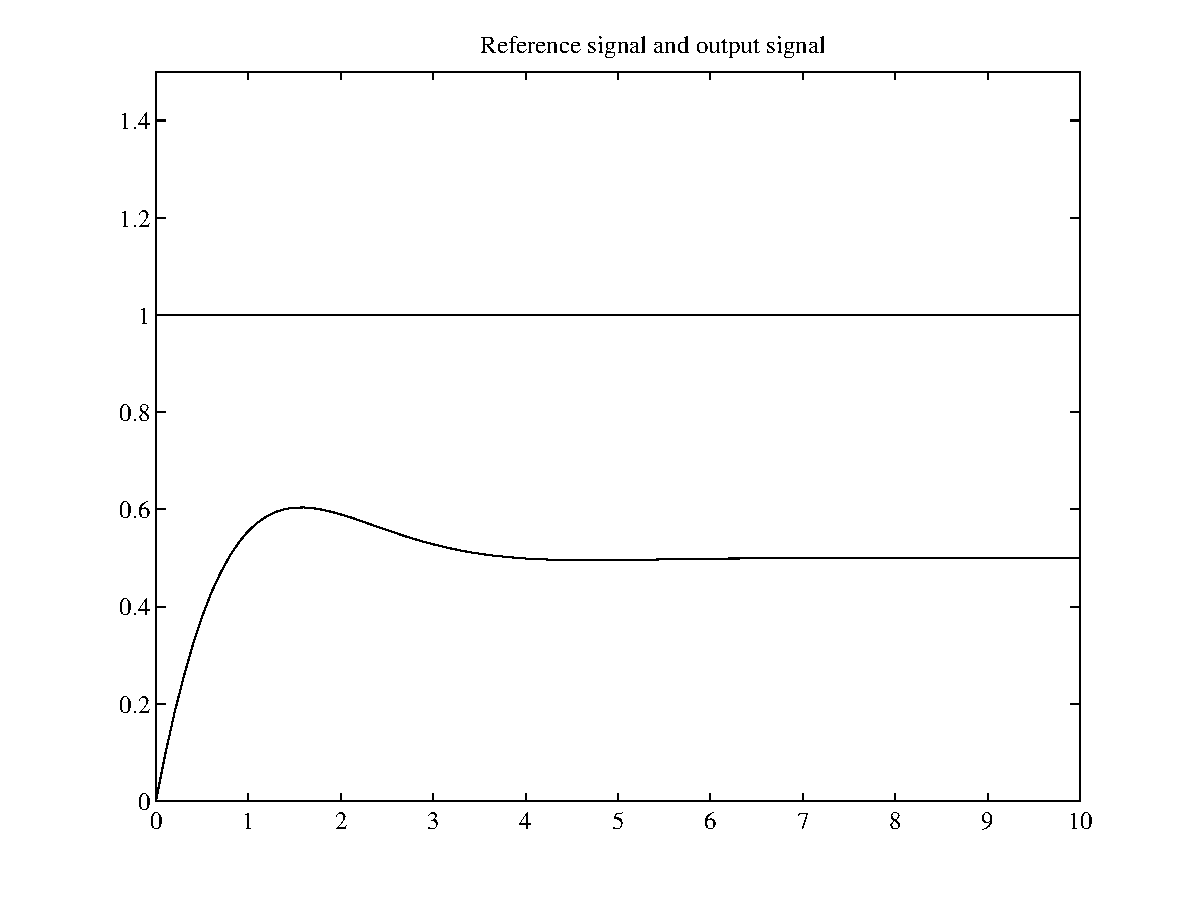
\includegraphics[width=0.48\linewidth]{../figures/fig930115-1a-1}
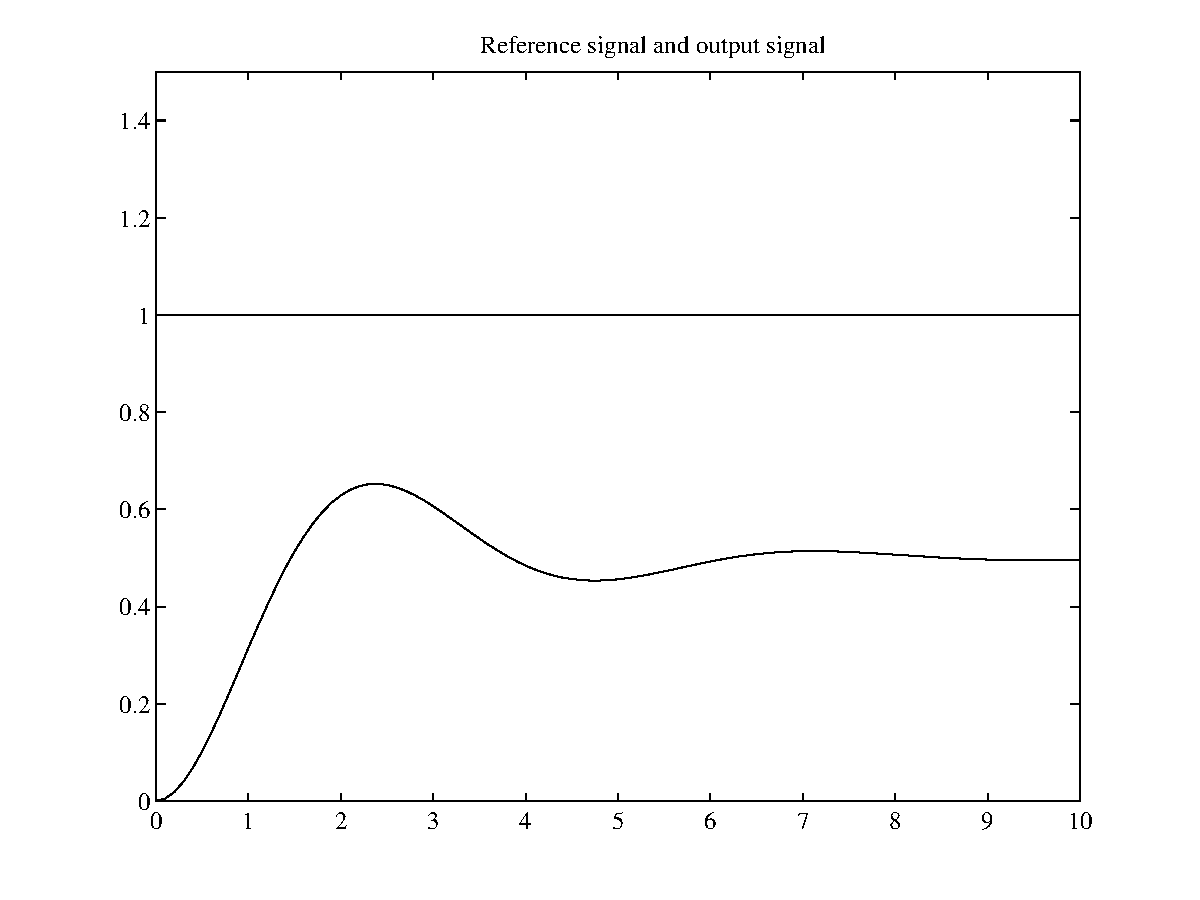
\includegraphics[width=0.48\linewidth]{../figures/fig930115-1a-2}\\
 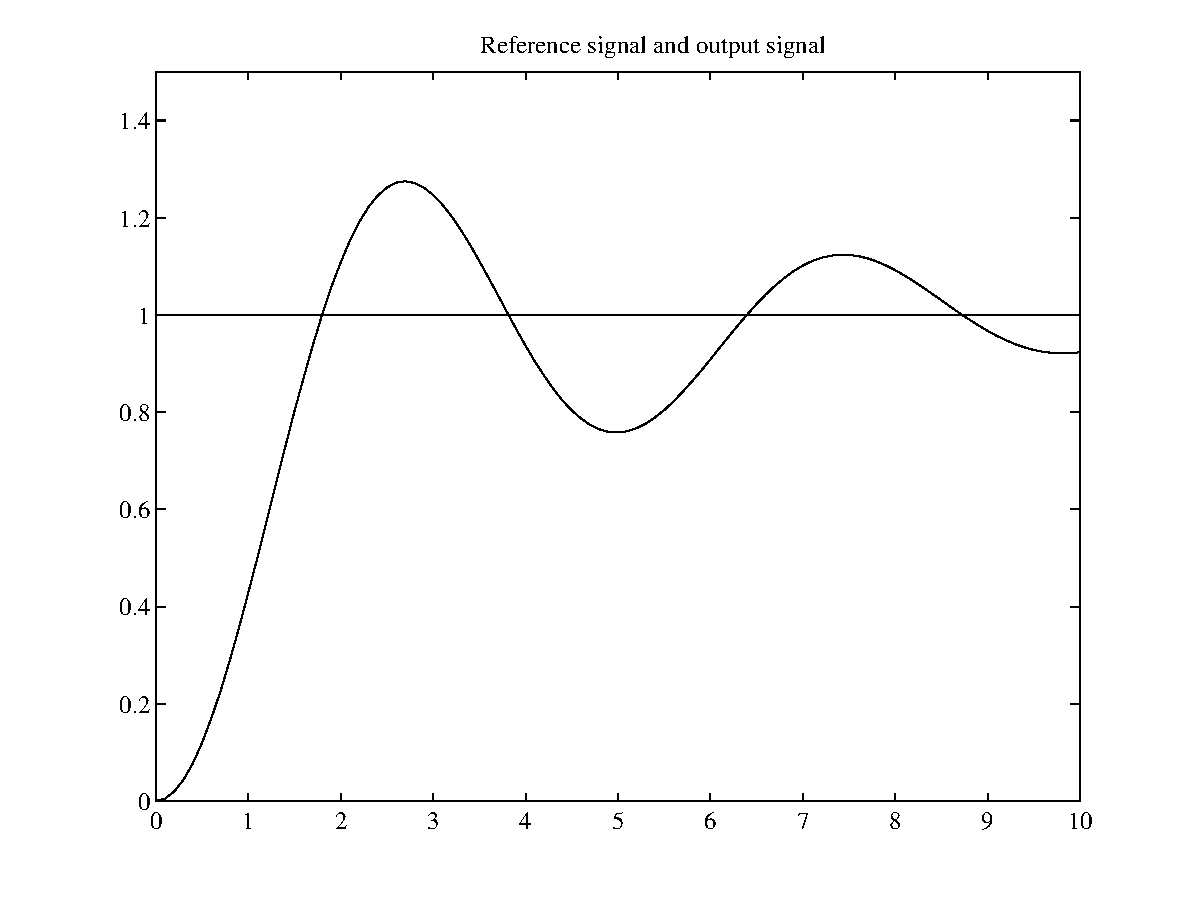
\includegraphics[width=0.48\linewidth]{../figures/fig930115-1a-3}
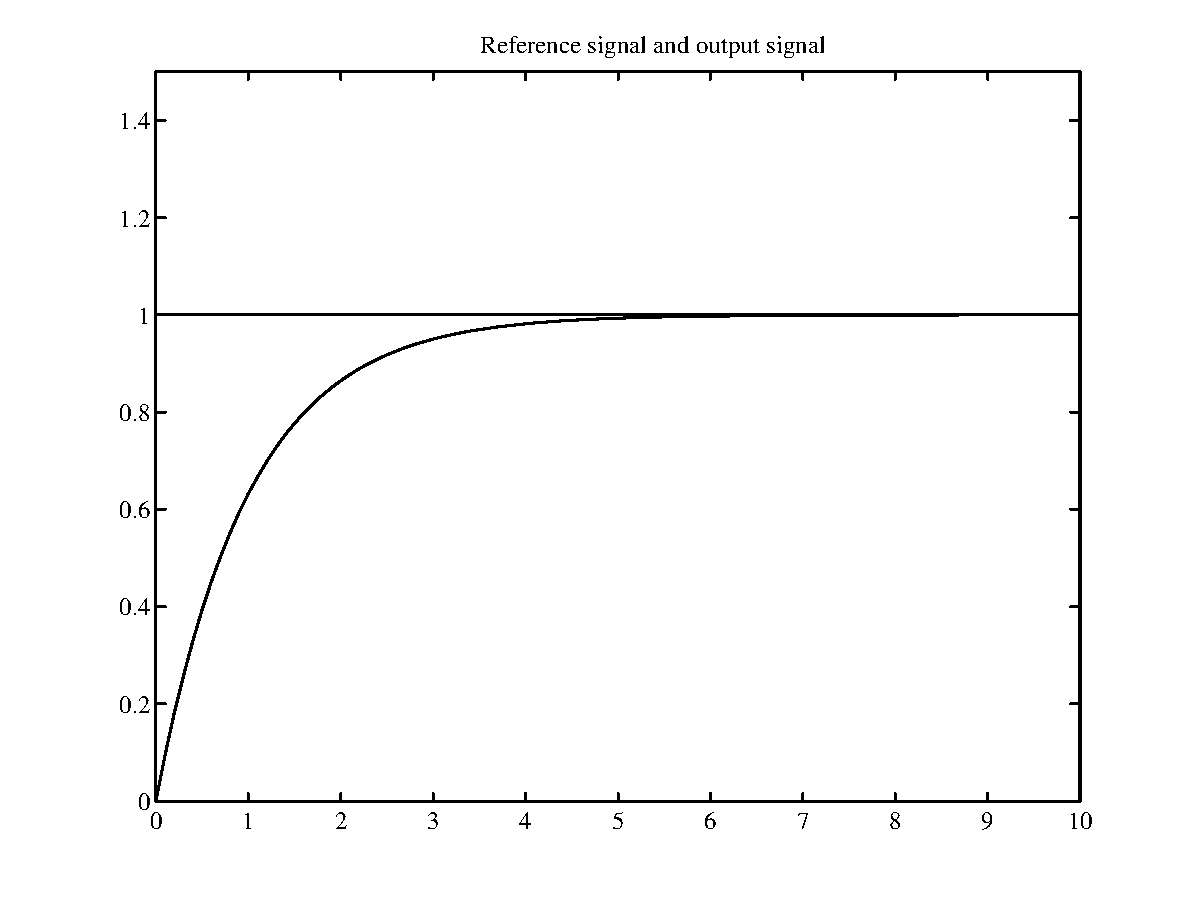
\includegraphics[width=0.48\linewidth]{../figures/fig930115-1a-4}
\end{center}

\section{Ziegler-Nichols ultimate gain tuning}
\label{sec-3}

Ziegler and Nichols developed their tuning rules for PID
regulators given that the system can be approximated as a first order system with time delay:
\( G(s) = \frac{e^{-sT}}{s+a} \).
We perform a resonance test according to Ziegler-Nichols' ultimate gain method and
with the proportional gain $K = 5 = K_u$ we get the closed-loop step response seen below
\begin{center}
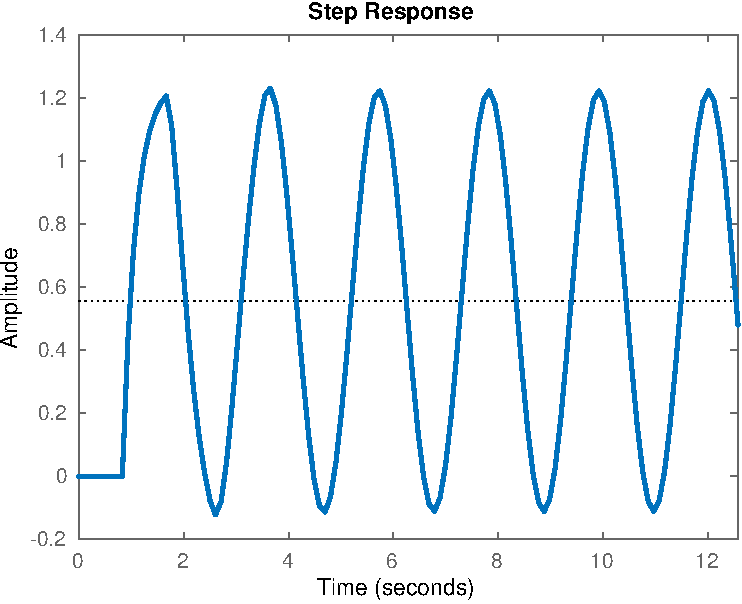
\includegraphics[width=0.4\linewidth]{../figures/zn_excercise_step-crop}
\end{center}
\begin{enumerate}
\item What is the period \(T_u\) and angular frequency \(\omega_u\) of the oscillations?
\item Determine the parameters  \(T\) and \(a\) in the transfer function \(G(s)\).
\item Tune a PI regulator \[u(t)=K_{p}\left(e(t)+{\frac{1}{T_{i}}}\int _{0}^{t}e(\tau )d\tau \right)\] according to Ziegler-Nichols' recipe.

\begin{center}
\begin{tabular}{llll}
Controller type & \(K_p\) & \(T_i\) & \(T_d\)\\
\hline
P & \(0.5 K_u\) &  & \\
PI & \(0.45 K_u\) & \(T_u/1.2\) & \\
PD & \(0.8 K_u\) &  & \(T_u/8\)\\
PID & \(0.6 K_u\) & \(T_u/2\) & \(T_u/8\)\\
\hline
\end{tabular}
\end{center}
\item The Nyquist plot of the resulting loop gain \(G_o(s) = F(s)G(s)\) is shown below. What are the stability margins?
\begin{center}
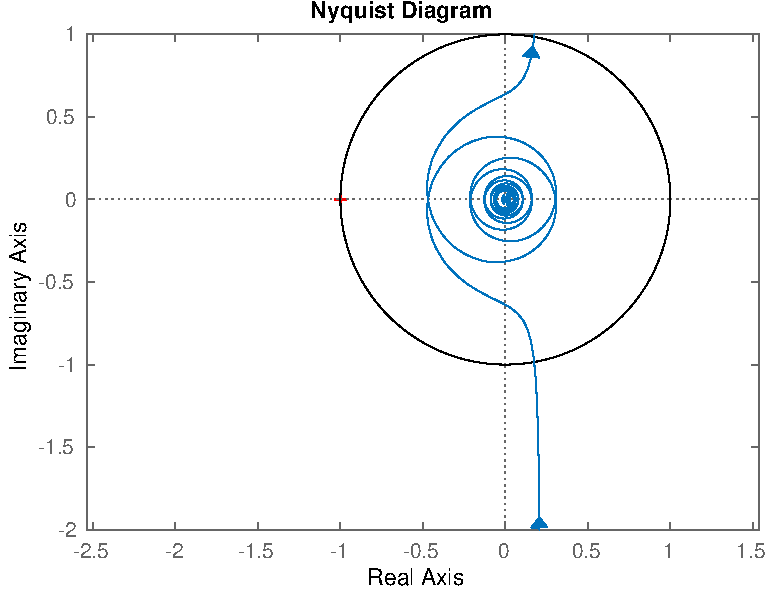
\includegraphics[width=0.5\linewidth]{zn_excercise_nyq-crop}
\end{center}
\item The cross-over frequency is \(\omega_c = \unit{0.39}{\rad\per\second}\) with the tuned PI controller. Determine a sampling period \(h\) for a discrete-time implementation of the PI controller, such that the phase margin is reduced by about \unit{10}{\degree}.
\end{enumerate}
% Emacs 24.5.1 (Org mode 8.2.10)
\end{document}